\subsection{Implementación mediante celdas enlazadas}
En esta implementación hacemos uso de memoria dinámica ya que no conocemos el número máximo de nodos que puede contener el árbol.

Vamos a ver dos propuestas de dicha implementación que son correctas pero muy ineficientes:
\begin{figure}[h]
  \begin{minipage}{0.55\textwidth}
    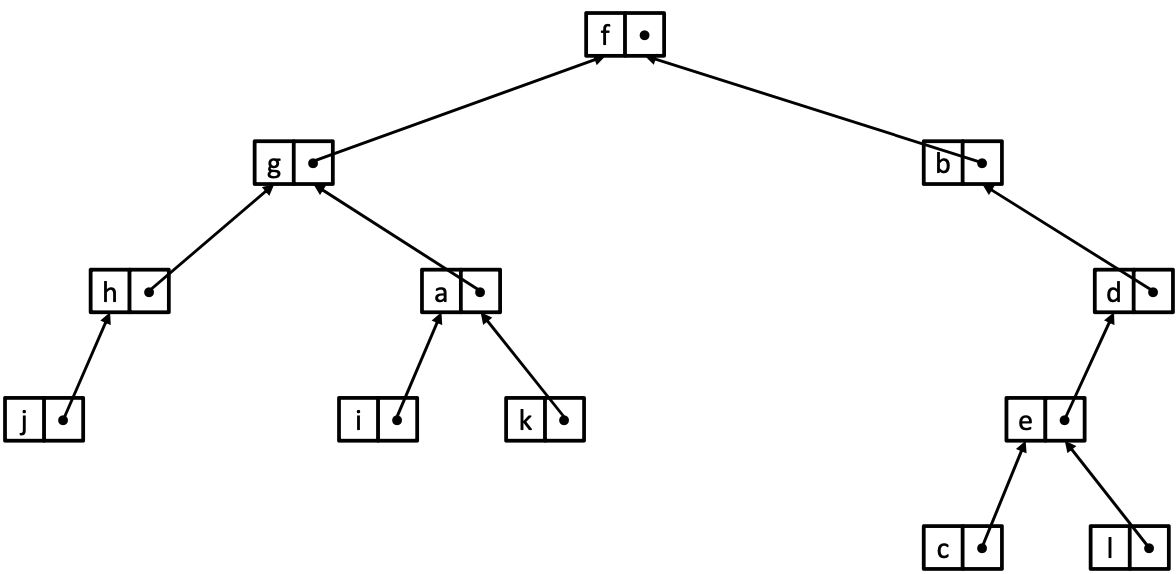
\includegraphics[width=0.8\textwidth]{assets/ICE1.png}
  \end{minipage}
  \hfill
  \begin{minipage}{0.4\textwidth}
    Esta implementación es muy costosa ya que es de orden \(O (n)\) y además al no tener acceso directo al nodo padre ni a los hijos tenemos que acceder desde las hojas, por tanto, al tener que acceder desde las hoja tenemos que recorrer el árbol entero.
  \end{minipage}
\end{figure}

\begin{figure}[h]
  \begin{minipage}{0.55\textwidth}
    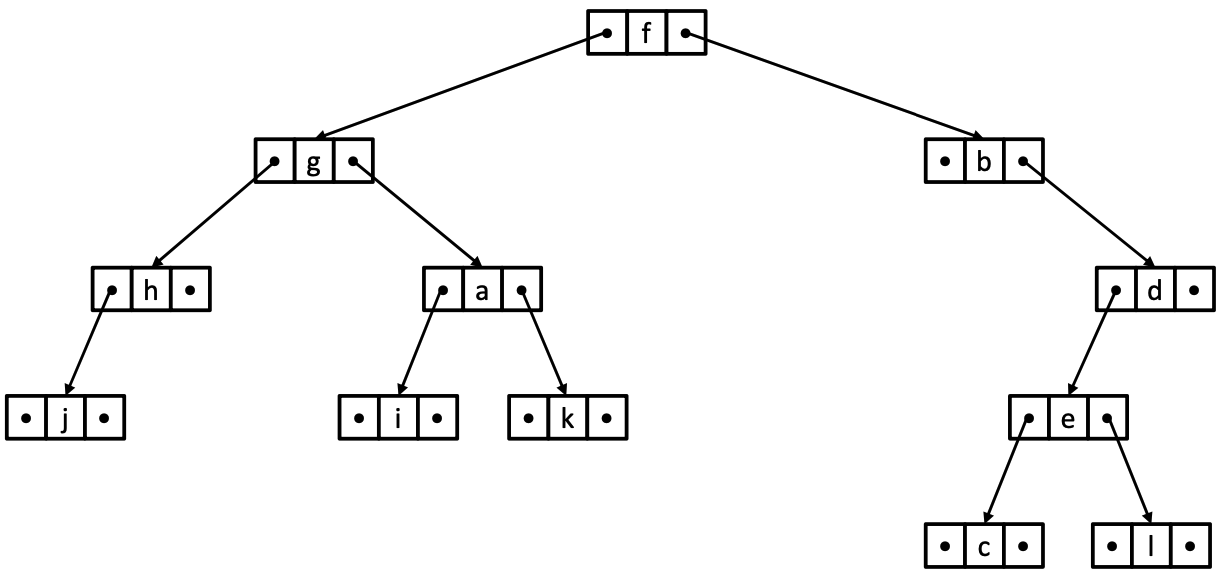
\includegraphics[width=0.8\textwidth]{assets/ICE2.png}
  \end{minipage}
  \hfill
  \begin{minipage}{0.4\textwidth}
    Esta implementación soluciona parcialmente el problema del acceso a los nodos (ya que si podemos acceder a los hijos) pero seguimos sin tener acceso al padre, por lo que su coste sigue siendo \(O (n)\).
  \end{minipage}
\end{figure}

\subsubsection*{Nuestra implementación del TAD árbol binario mediante celdas enlazadas}
\begin{figure}[h]
  \begin{center}
    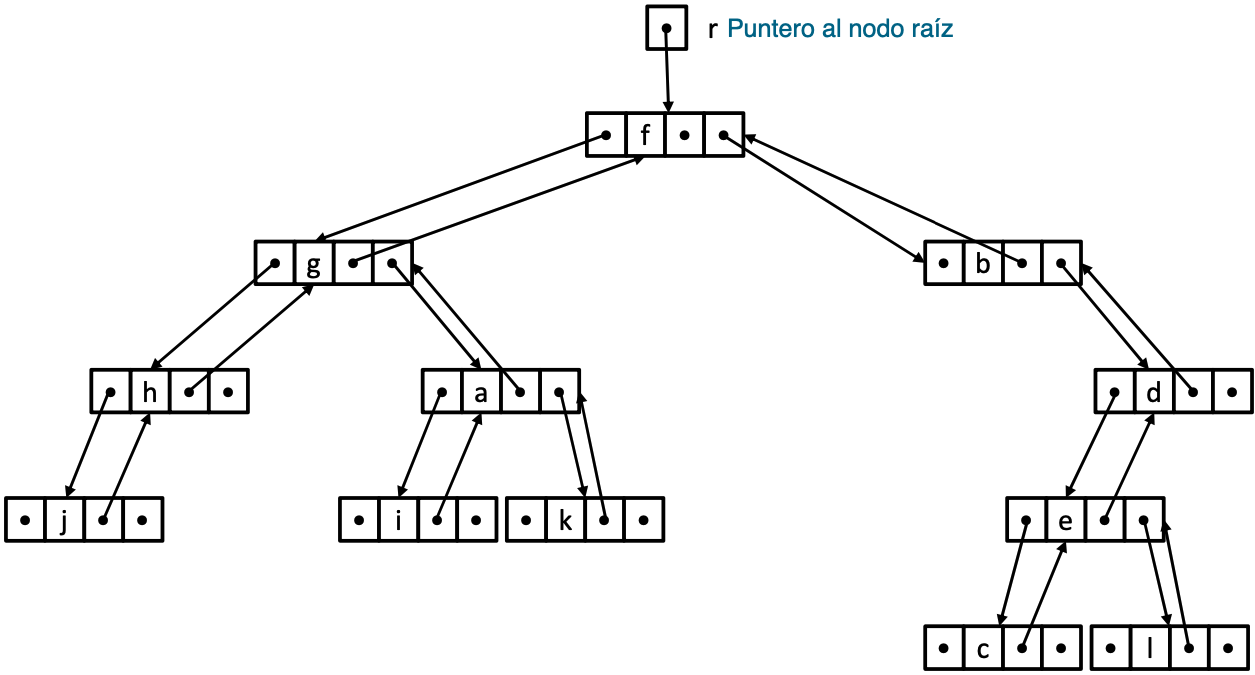
\includegraphics[width=0.8\textwidth]{assets/ICE3.png}
  \end{center}
\end{figure}
Esta será nuestra implementación de dicho TAD, debido a que se corrigen todos los problemas descritos anteriormente, ahora tenemos acceso directo al nodo raíz y podemos acceder a cualquer nodo del árbol.

Finalmente, vemos que gracias a esta implementación todas las operaciones del TAD pasan a ser de orden \(O(1)\).

En memoria se almacenará celdas cuyo contenido son los nodos (padre, hijo izquierdo y derecho) y el elemento del mismo (si ese nodo es nulo, no hay celda), por tanto, en la parte privada del TAD tendremos:
\begin{minted}[breaklines]{C++}
template <typename T> class Abin{
  public:
    //Métodos vistos en la especificación del TAD
  private:
    struct celda{
      T elto; //elemento del nodo
      nodo padre, hizq, hder; //nodos
      celda(const T& e, nodo p = NODO_NULO):elto(e),padre(p),
      hizq(NODO_NULO),hder(NODO_NULO){}
    };
    nodo r; //nodo raíz del árbol.
};
\end{minted}
\subsubsection*{Notas sobre el código de la implementación del TAD}
En la parte pública de la clase encontramos:\\
\verb|  static const nodo NODO_NULO;|, que nos va a permitir indicar explicitamente la no existencia de un nodo.

A la hora de construir un Abin, este se debe de crear vacío, es decir, el nodo raíz es un nodo nulo:\\
\verb|  template <typename T> inline Abin<T>::Abin():r(NODO_NULO){}|

Cuando vayamos a insertar el nodo que será la raíz del árbol solo le pasamos el contenido del mismo, ya que al tener un puntero a la raíz no nos hace falta pasarle el nodo:
\begin{minted}[breaklines]{C++}
template <typename T> inline void Abin<T>::insertarRaiz(const T& e){
  assert(r == NODO_NULO); //Comprobamos la Precondición
  r = new celda(e); //Inserción del nodo raíz.
}
\end{minted}

Si queremos insertar ya sea un nodo hijo izquierdo o derecho, tenemos que pasarle el nodo n (padre de ese nuevo nodo) y el elemento del nodo a insertar.
\begin{minted}[breaklines]{C++}
template <typename T> inline void Abin<T>::insertarHijoIzqdo(nodo n, const T& e){
  //Comprobamos Precondiciones
  assert(n == NODO_NULO); 
  assert (n->hizq ==NODO_NULO);
  n->hizq = new celda(n,e); //Inserción del nodo hijo izquierdo de n.
}
\end{minted}
\textit{NOTA:} Análogamente para la inserción del hijo derecho de un nodo.

Si queremos eliminar un nodo, este debe ser una hoja. Por tanto, primero debemos comprobar si el nodo es una hoja. Si lo es, lo eliminamos dejándolo como un nodo nulo. Esto asegura que el nodo quede en un estado válido y que la dirección de memoria que ocupa la celda se libere correctamente.
\begin{minted}[breaklines]{C++}
template <typename T> inline void Abin<T>::eliminarHijoIzqdo(nodo n){
  //Comprobamos Precondiciones
  assert(n==NODO_NULO);
  assert(n->hizq!=NODO_NULO);//existe hijo izquierdo
  assert(n->hizq->hizq==NODO_NULO && n->hizq->hder==NODO_NULO); //Es Hoja

  //Lo explicado anteriormente
  delete n->hizq; //eliminamos
  n->hizq = NODO_NULO; //lo dejamos en estado válido
}
\end{minted}
\textit{NOTA:} No podemos hacer estos dos últimos paso a la inversa debido a que si lo dejamos como estado válido (nodo nulo), no podremos eliminar el puntero ni la dirección de memoria.
\textit{NOTA:} Análogamente para la eliminación del hijo derecho de un nodo.

Por otro lado, encontramos si queremos eliminar la raíz de un árbol, esta debe de ser una hoja, y por ende al ser eliminado dicho nodo el árbol quedaría vacío.
\begin{minted}[breaklines]{C++}
template <typename T> inline void Abin<T>::eliminarRaiz(){
  //Comprobamos Precondiciones
  assert(r == NODO_NULO);
  assert(r->hizq == NODO_NULO && r->hder == NODO_NULO);
  delete r;
  r = NODO_NULO;
}
\end{minted}

Dentro de la parte privada del TAD encontramos dos métodos:
\begin{itemize}
  \item \verb|DestruirNodos(nodo& n)|; donde dado un nodo n elimina todos los descendientes del mismo, para poder eliminar al mismo. Esto nos simplifica mucho el destructor de la clase ya que al ser un método recursivo se ejecuta tantas veces hasta que llega a la condición de parada `NODO\_NULO'.
  \begin{minted}[breaklines]{C++}
template <typename T> void Abin<T>::destruirNodos(nodo& n){
  if(n!= NODO_NULO){
    destruirNodos(n->hizq);
    destruirNodos(n->hder);
    delete n;
    n=NODO_NULO;
  }//Para cuando n = NODO_NULO
}
  \end{minted}
  \item \verb|Copiar(nodo n)|; dado un nodo n cualquiera realiza una copia de dicho nodo y todos sus descendientes, donde ese nodo n es la raíz del nuevo árbol creado.
  \begin{minted}[breaklines]{C++}
template <typename T> typename Abin<T>::nodo Abin<T>::copiar(nodo n){
  nodo m = NODO_NULO; //creamos un nodo m aux
  if(n!= NODO_NULO){
    m = new celda(n->elto); //copiamos el padre (n).
    m->hizq = copiar(n->hizq); //copiamos subárbol izquierdo recursivamente
    if(m->hizq != NODO_NULO)
      m->hizq->padre = m;
    m->hder = copiar(n->hder); //copiamos subárbol derecho recursivamente
    if(m->hder != NODO_NULO)
      m->hder->pader = m;
  }
  return m;
}
  \end{minted}
\end{itemize}